\documentclass[titlepage]{jsarticle}
\usepackage[dvipdfmx]{graphicx}
\usepackage{listings}
\usepackage{cprotect}
\usepackage{h31ec-exp}
\lstset{
  basicstyle={\ttfamily},
  identifierstyle={\small},
  commentstyle={\smallitshape},
  keywordstyle={\small\bfseries},
  ndkeywordstyle={\small},
  stringstyle={\small\ttfamily},
  frame={tb},
  breaklines=true,
  columns=[l]{fullflexible},
  numbers=left,
  xrightmargin=0zw,
  xleftmargin=3zw,
  numberstyle={\scriptsize},
  stepnumber=1,
  numbersep=1zw,
  lineskip=-0.5ex
}
\renewcommand{\lstlistingname}{ソースコード}
\makeatletter
\newcommand{\figcaption}[1]{\def\@captype{figure}\caption{#1}}
\newcommand{\tblcaption}[1]{\def\@captype{table}\caption{#1}}
\makeatother
\title{信号処理プログラミング}
\grade{4年32番}
\author{平田 蓮}
\team{}
\date{2020年6月18日}
\expdate{2020年5月21日, 5月28日, 6月4日, 6月11日}
\coauthor{
}

\begin{document}
\maketitle
\section{目的}
    アナログ信号をディジタルデータに変換し, ディジタル機器で処理するために必要な起訴事項について学習し,
    C言語で基本的な信号処理プログラムを作成する.
    また音声フォーマットの一つであるWAVEファイルの構造を理解し, 音声データの入出力プログラムを作成する.

\section{周期関数の生成と可視化}
    正弦波のように一定周期ごとに同じ波形が繰り返される関数を\textbf{周期関数}と呼ぶ.
    よく知られている周期関数として, のこぎり波などがある.
    本節では周期関数に関する演習を行う.

    \paragraph{演習1-1} 任意の孤度$r$を区間$[0:2\pi]$に変換する関数\verb|rad|を作成せよ.

        作成した関数をソースコード\ref{src:rad}に示す.

        \begin{lstlisting}[caption=rad.c, label=src:rad]
double rad(double r) {
    if (r >= 0) {
        return fmod(r, 2 * PI);
    } else {
        return 2 * PI - fmod(-r, 2 * PI);
    }
}
        \end{lstlisting}

        $r$が正のときは$2\pi$との剰余を取る.
        $r$が負のときは, $r$を正数に変換し, $2\pi$と剰余をとったものを$2\pi$から引くことで変換している.

        図\ref{fig:rad}に横軸に$r$, 縦軸に\verb|rad(r)|を取ったグラフを示す.
        この図から, 変換がうまく行われていることがわかる.

        \begin{figure}[ht]
            \centering
            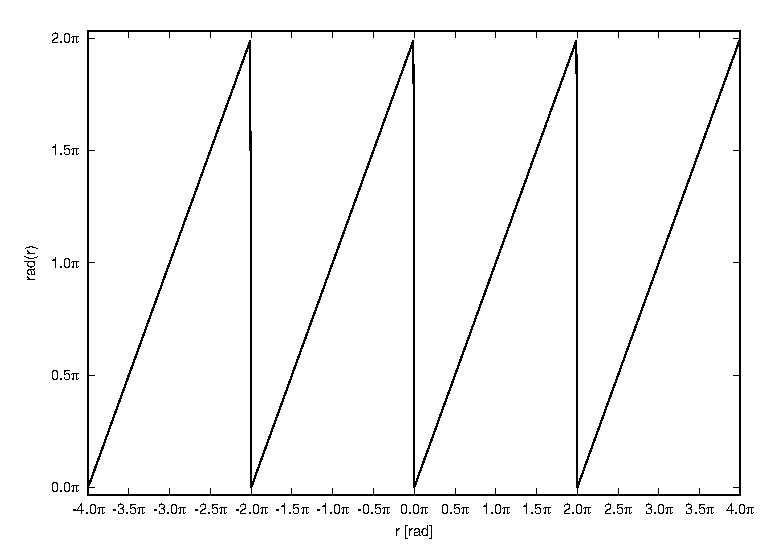
\includegraphics[width=12cm]{images/rad.eps}
            \cprotect\caption{\verb|rad|による変換}
            \label{fig:rad}
        \end{figure}

    \paragraph{演習1-2} 任意の孤度$r$に対して, のこぎり波の振幅値を求める関数\verb|saw|を作成せよ.

        作成した関数をソースコード\ref{src:saw}に示す.

        \begin{lstlisting}[caption=saw.c, label=src:saw]
double saw(double r) {
    return 1 - rad(r) / PI;
}
        \end{lstlisting}

        まず与えられた孤度$r$を演習1-1で実装した\verb|rad|を使い$[0:2\pi]$の範囲に変換する.

        $r$が$2\pi$の倍数の場合に1を取り, そこから傾き$-\frac{1}{\pi}$の形を繰り返すので,
        上記のように実装することができた.

        図\ref{fig:saw}にグラフを示す. うまくのこぎり波が現れていることがみてとれる.

        \begin{figure}[ht]
            \centering
            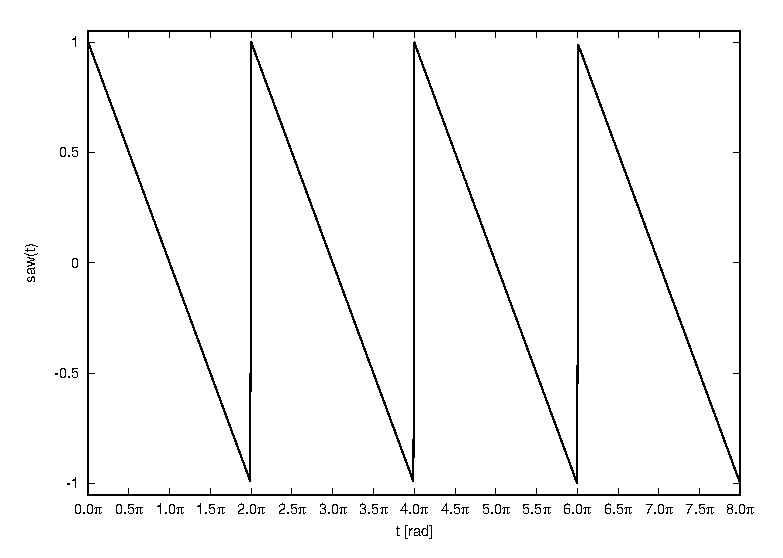
\includegraphics[width=12cm]{images/saw.eps}
            \cprotect\caption{\verb|saw|による変換}
            \label{fig:saw}
        \end{figure}

\section{サンプリング}
    アナログ信号波形をディジタルデータに変換する手法に\textbf{サンプリング}がある.
    本節では演習問題を通して実際にサンプリングの様子を観察する.

    \paragraph{演習2-1} リスト2のコードを解析し, 完成させよ. 振幅100, 周波数4Hzのデータを
    出力リダイレクションを使ってsin100f4.csvに出力せよ. このsin100f4.csvをgnuplotでグラフ化し,
    サンプリングの効果を確認せよ.

        まず, 完成させたリスト2のコード, sin10af1.cを出力部分を抜粋して掲載する.

        \begin{lstlisting}[caption=sin10af1.c, label=src:sin10af1]
int t;
double amp, frq, rad, vin;
unsigned char vout;

for (t = 0; t <= TEND; t += DT) {
    rad = 2 * PI * frq * t / 1000.0;
    vin = amp * sin(r) + BIAS;
    if (vin > 255) {
        vout = 255;
    } else if (vin < 0) {
        vout = 0;
    } else {
        vout = vin;
    }
    printf("%4f, %4d\n", t / 1000.0, vout);
}
        \end{lstlisting}

        4行目から10行目に渡って, クリッピングという処理を施してある.
        クリッピングをすることで, 出力用の変数(今回は8bitのchar型)に収まらない値を切り捨て,
        波形を維持することができる.

        図\ref{fig:sin100f4}にサンプリングしたデータを示す.
        実際に正弦波をサンプリングできていることがわかる.

        \begin{figure}[ht]
            \centering
            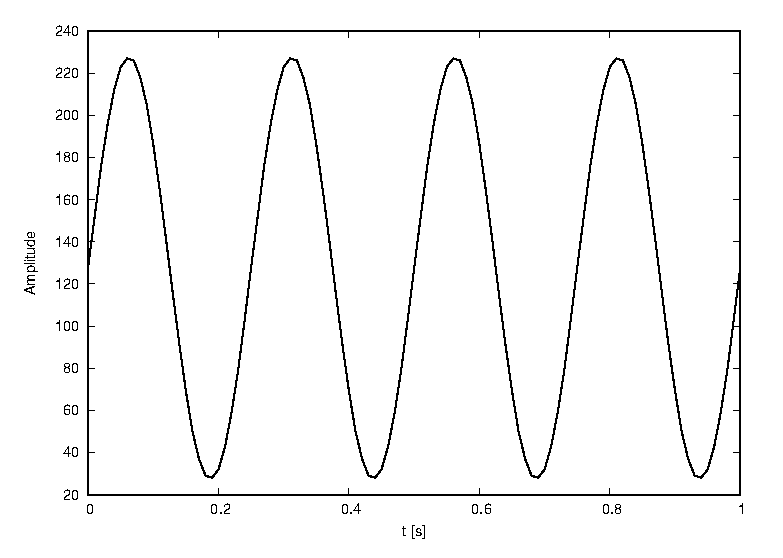
\includegraphics[width=12cm]{images/sin100f4.eps}
            \caption{振幅100, 周波数4Hzの正弦波}
            \label{fig:sin100f4}
        \end{figure}

    \paragraph{演習2-2} 振幅150, 周波数4Hzのデータsin150f4.csvを生成しその波形を確認せよ.
    波形に不具合があればその原因を考えて不具合を軽減するような修正を行え.
        
        今回は振幅が150なので, char型に収まらない数値をサンプリングすることになる.
        そこで, 演習2-1で実装したクリッピングが働く.

        図\ref{fig:sin150f4}にクリッピングを施した前と後の波形を示す.
        この図からクリッピングの効果がみて取れる.
        点線のクリッピングをしていない波形では, オーバーフローした値が波形の逆側に飛んでしまい,
        波形が崩れているが, 実線のクリッピングを施した方ではオーバーフローした値が切り捨てられ, 波形が維持できている.
        
        \begin{figure}[ht]
            \centering
            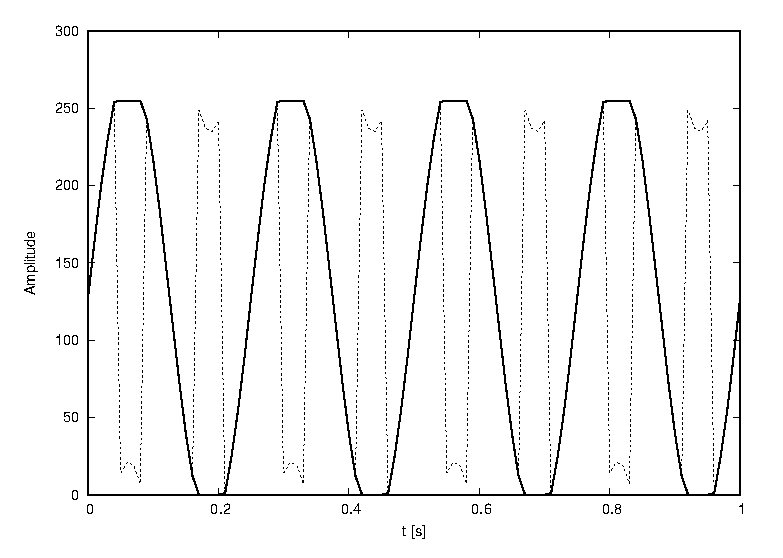
\includegraphics[width=12cm]{images/sin150f4.eps}
            \caption{振幅150, 周波数4Hzの正弦波}
            \label{fig:sin150f4}
        \end{figure}

    \paragraph{演習2-5} サンプリング定理を満たさないような高い周波数の正弦波をPCMによりディジタルデータ化すると,
    周波数や位相が全く異なる波形に見えることがある. この現象を実際に観察せよ.

        今回はサンプリング周波数が100Hzであるので, 50Hzを超える周波数の波はうまくサンプリングをすることができない.

        試しに98Hzの波形をサンプリングしてみると実際には98Hzであるはずが, 2Hzの波形のように見える.
        これは, 実際には一周期以上波形が進んでいるが, サンプリングするときは少しの変化として認識しまっているためである.
        
        参考に, 上の波形にサンプリング周波数を上げて計測した本来の98Hzの波形を重ねたものを図\ref{fig:sin98}に示す.

        \begin{figure}[ht]
            \centering
            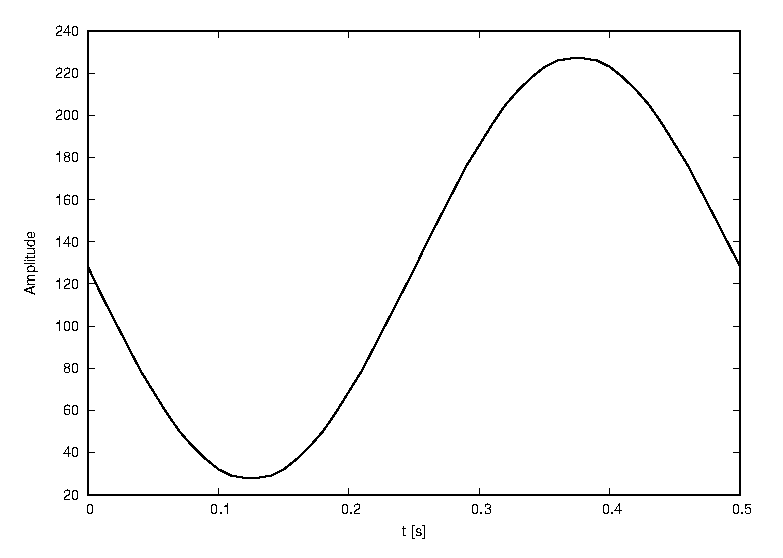
\includegraphics[width=12cm]{images/sin98.eps}
            \caption{周波数98Hzの正弦波}
            \label{fig:sin98}
        \end{figure}

\section{信号処理プログラムの分類}
    信号処理プログラムは, オンライン型をオフライン型の二種類に分類することができる.
    データを一つ取り込むたびに逐次処理を行うオンライン型に対して,
    オフライン型はデータを一定数取り込んだの後に一括処理を行う.

\section{雑音除去}
    信号に重畳された雑音を取り除く処理は, 極めて基本的な信号処理である.
    演習3では雑音の処理に関する演習を行う.

    \paragraph{演習3-1} リスト3を参考に, コマンドライン引数で元信号のCSVファイルと,
    白色雑音の最大振幅を与えたとき, 白色雑音を加えるオフライン型のプログラムadd-wn2.cを作成せよ.

        作成したプログラムの信号処理部分を抜粋してソースコード\ref{src:wn}に示す.

        \begin{lstlisting}[caption=add-wn2.c, label=src:wn]
double tm[DATANUM];
int amp[DATANUM], nmax;
double err;

for (int n = 0; n <= DATANUM; n++) {
    err = nmax * (2.0 * rand() / RAND_MAX - 1.0);
    amp[n] += ROUND(err);

    printf("%4d, %4d\n", tm[n], amp[n]);
}
        \end{lstlisting}

        通常のsin波に最大振幅10の白色雑音を加えたものを図\ref{fig:sin_wn}に示す.
        点線が元の正弦波で, 雑音が加えられたものが実線で描いてある.
        図から, 適当な雑音が加えられていることがわかる.

        \begin{figure}[ht]
            \centering
            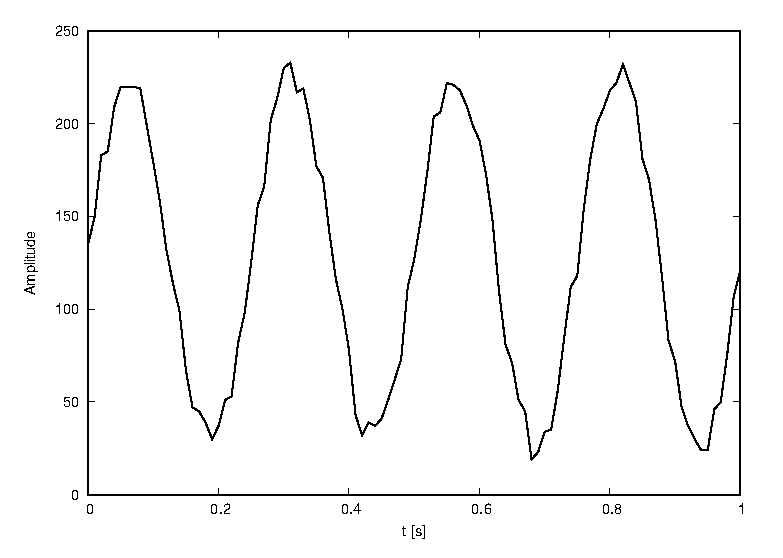
\includegraphics[width=12cm]{images/sin_wn.eps}
            \caption{最大振幅10の正弦波を加えたsin波}
            \label{fig:sin_wn}
        \end{figure}

    \paragraph{演習3-2} 3点単純移動平均プログラムmvave3-?.cを作成せよ(?はオンライン型は1,
    オフライン型は2).

        図\ref{src:mvave_1}, \ref{src:mvave_2}にそれぞれオンライン型とオフライン型のソースコードを抜粋して示す.

        \begin{lstlisting}[caption=mvave3-1.c, label=src:mvave_1]
int tm, __amp = 0, _amp = 0, amp, _tm;

while (fgets(buf, sizeof(buf), fp) != NULL) {
    if (buf[0] == '#') continue;
    
    tm  = atoi(strtok(buf, ","));
    amp = atoi(strtok(NULL, "\r\n\0"));

    if (_amp == 0) {
        _amp = amp;
        continue;
    }
    if (__amp == 0) {
        __amp = _amp;
        _tm = tm;
        continue;
    }

    vout = ROUND((__amp + _amp + amp) / 3.0);
    printf("%4d, %4d\n", _tm, (int)vout);

    __amp = _amp;
    _amp  = amp;
    _tm   = tm;
}
        \end{lstlisting}
        \begin{lstlisting}[caption=mvave3-2.c, label=src:mvave_2]
for (int n = 1; n < DATANUM; n++) {
    vout = ROUND((amp[n - 1] + amp[n] + amp[n + 1]) / 3.0);

    printf("%4d, %4d\n", tm[n], (int)vout);
}
        \end{lstlisting}

        オンライン型のソースコードでは, 3点平均を計算するために2個前までのデータ,
        また, 出力用に一個前のtを毎回更新している.

        これらのプログラムで図\ref{fig:sin_wn}から雑音を取り除いた波形を図\ref{fig:mvave}に示す.

        \begin{figure}[ht]
            \centering
            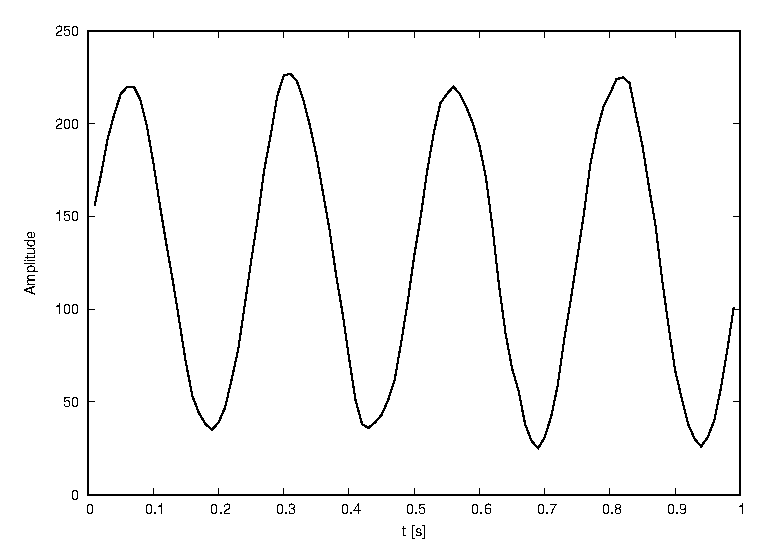
\includegraphics[width=12cm]{images/mvave.eps}
            \caption{雑音を取り除いた波形}
            \label{fig:mvave}
        \end{figure}

        3点平均を取る過程で始点と終点のデータが一つずつ欠けてしまっているが,
        波形は概ね元のものに近づいている.

\section{時系列データの解析}
    周期的なアナログ信号$x(t)$に由来する時系列データ$x_i;i=1,2,\dots,N$が与えられたとき,
    元の信号の基本周波数, 振幅, 位相などを求めることを信号解析を呼ぶ.
    本実験では信号の\textbf{最小値}, \textbf{最大値}, \textbf{平均値}, \textbf{標準偏差}, \textbf{最大振幅}, \textbf{実効値}を求める.

    \paragraph{平均値と標準偏差} 時系列データ$x_i;i=1,2,\dots,N$の平均値$\bar{x}$は次式で定義される:
        
        \begin{equation} \label{eqn:mean}
            \bar{x} = \frac{1}{N} \sum_{i=1}^{N} x_i
        \end{equation}

        標準偏差$\sigma$は分散$\sigma^2$の正の平方根として定義される:
        
        \begin{equation} \label{eqn:dev1}
            \sigma^2 = \frac{1}{N} \sum_{i=1}^{N} (x_i - \bar{x})^2
        \end{equation}

        この式では平均値が既知である必要があり, オンライン処理に適用することができない.
        オンライン処理で標準偏差や分散を計算したい場合は, 変形した次式を用いる:

        \begin{equation} \label{eqn:dev2}
            \sigma^2 = \frac{1}{N} \sum_{i=1}^{N} x_i^2 - \bar{x}^2
        \end{equation}

    \paragraph{演習4-1} 式(\ref{eqn:dev1})を式(\ref{eqn:dev2})に変形する過程を示せ.
        
        \begin{eqnarray*}
            \sigma^2 &=& \frac{1}{N} \sum_{i=1}^{N} (x_i - \bar{x})^2 \\
            &=& \frac{1}{N} \sum_{i=1}^{N} (x_i^2 - 2x_i \bar{x} + \bar{x}^2) \\
            &=& \frac{1}{N} \sum_{i=1}^{N} x_i^2 - \frac{2}{N} \bar{x} \sum_{i=1}^{N} x_i + \frac{\bar{x}^2}{N} \sum_{i=1}^{N} 1 \\
        \end{eqnarray*}

        式(\ref{eqn:mean})より, $\frac{2}{N} \bar{x} \sum_{i=1}^{N} x_i = 2 \bar{x}^2$なので,

        \begin{eqnarray*}
            \sigma^2 &=& \frac{1}{N} \sum_{i=1}^{N} x_i^2 - \frac{2}{N} \bar{x} \sum_{i=1}^{N} x_i + \frac{\bar{x}^2}{N} \sum_{i=1}^{N} 1 \\
            &=& \frac{1}{N} \sum_{i=1}^{N} x_i^2 - 2 \bar{x}^2 + \bar{x}^2 \\
            &=& \frac{1}{N} \sum_{i=1}^{N} x_i^2 - \bar{x}^2 \\
        \end{eqnarray*}

    \paragraph{演習4-2} コマンドライン引数で与えられたCSVファイルについて, 最小値, 最大値, 平均値,
    標準偏差, 最大振幅, 実効値を求めるプログラムstat?.cを作成せよ(?はオンライン型は1,
    オフライン型は2).

        作成したプログラムをソースコード\ref{src:stat1}, \ref{src:stat2}に示す.

        \begin{lstlisting}[caption=stat1.c, label=src:stat1]
int tm, amp;
char buf[BUFSIZE];
double
    min_val = INF, max_val = -INF,
    sum = 0, mean, sum_squ = 0,
    std_dev, data_num = 0, max_amp, rms = 0;
FILE *fp;

while (fgets(buf, sizeof(buf), fp) != NULL) {
    if (buf[0] == '#') continue;

    data_num += 1;
    
    tm  = atoi(strtok(buf, ","));
    amp = atoi(strtok(NULL, "\r\n\0"));

    if (min_val > amp) min_val = amp;
    if (max_val < amp) max_val = amp;

    sum += amp;

    sum_squ += amp * amp;

    rms += amp - BIAS;
}
fclose(fp);

mean = sum / data_num;
std_dev = sqrt(sum_squ / data_num -  mean * mean);

if (BIAS - min_val > max_val - BIAS) {
    max_amp = BIAS - min_val;
} else {
    max_amp = max_val - BIAS;
}

rms = sqrt(sum_squ / data_num - 2 * mean * max_amp + max_amp * max_amp);

printf(
    "Min: %f, Max: %f, Mean: %f, Std Deviation: %f, Max Amplitude: %f, RMS: %f\n",
        min_val, max_val, mean,     std_dev,           max_amp,           rms
);
        \end{lstlisting}
        \begin{lstlisting}[caption=stat2.c, label=src:stat2]
int tm[DATANUM], amp[DATANUM];
char buf[BUFSIZE];
double
    min_val = INF, max_val = -INF,
    sum = 0, mean, sum_squ = 0, std_dev,
    data_num = 0, max_amp, rms;
FILE *fp;

for (int n = 0; n <= DATANUM; n++) {
    if (min_val > amp[n]) min_val = amp[n];
    if (max_val < amp[n]) max_val = amp[n];

    sum += amp[n];

    sum_squ += amp[n] * amp[n];

    rms += amp - BIAS;
}

mean = sum / data_num;
std_dev = sqrt(sum_squ / data_num -  mean * mean);

if (BIAS - min_val > max_val - BIAS) {
    max_amp = BIAS - min_val;
} else {
    max_amp = max_val - BIAS;
}

rms = sqrt(sum_squ / data_num - 2 * mean * max_amp + max_amp * max_amp);

printf(
    "Min: %f, Max: %f, Mean: %f, Std Deviation: %f, Max Amplitude: %f, RMS: %f\n",
        min_val, max_val, mean,     std_dev,           max_amp,           rms
);
        \end{lstlisting}

        試しに, 図\ref{fig:sin100f4}のデータを入力した時のデータを表\ref{tab:stat}にまとめる.

        \begin{table}[ht]
            \centering
            \caption{sin波の解析}
            \label{tab:stat}
            \begin{tabular}{c|c|c}
                項目 & 測定値 & 理論値 \\ \hline \hline
                最小値 & 28 & 28 \\ \hline
                最大値 & 227 & 228 \\ \hline
                平均値 & 127.5 & 128 \\ \hline
                標準偏差 & 70.42 & 70.71 \\ \hline
                最大振幅 & 100 & 100 \\ \hline
                実効値 & 75.61 & 70.71
            \end{tabular}
        \end{table}

        若干の誤差が見受けられるものの, ある程度の精度の値が出ている.
        誤差の原因として考えられるのは, サンプリング周波数の関係で最大値が測定できていないことなどがある.

\section{Windows WAVEファイルの解析$\cdot$加工}
    この節では, Windows標準のサウンドフォーマットであるWAVEファイルを,
    自作のCプログラムで読み書きをする.

\begin{thebibliography}{99}
    \bibitem{Electro} Electro-ワンチップマイコン http://laboratory.sub.jp/ele/13.html/
\end{thebibliography}

\end{document}
